\documentclass[11pt]{article}

\usepackage[a4paper,margin=2.6cm]{geometry}
\usepackage[T1]{fontenc}
\usepackage[utf8]{inputenc}
\usepackage{lmodern}
\usepackage{microtype}
\usepackage{amsmath,amssymb}
\usepackage{booktabs}
\usepackage{graphicx}
\usepackage{xcolor}
\usepackage[font=small,labelfont=bf]{caption}
\usepackage{enumitem}
\definecolor{linkblue}{HTML}{1c5cab}
\usepackage[colorlinks=true,linkcolor=linkblue,citecolor=linkblue,urlcolor=linkblue]{hyperref}

\newcommand{\sillage}{\textsc{Sillage}}
\newcommand{\dnll}{\Delta\mathrm{NLL}}
\newcommand{\ci}[2]{{\footnotesize[#1,\,#2]}}

\title{\bfseries One Signal, Three Tiers:\\
A Routed Memory Hierarchy with Surprise-Gated Consolidation\\
for Frozen Language Models}
\author{Abderrahmane Sghairi\\
\small Independent Researcher, Issoire, France\\
\small \texttt{sghairipro63@gmail.com}}
\date{August 2026}

\begin{document}
\maketitle

\begin{abstract}
Two companion systems gave frozen language models gradient-free memory: a fixed-size Hebbian matrix with $n$-gram keys and surprise-gated amplitude writes (\sillage{}), and a score-level router adding whitened-SimHash semantic keys. Their benchmarks also mapped, without intending to, the regimes of three \emph{different} memory mechanisms: the fast Hebbian tiers dominate fresh and bounded settings, an exact $n$-gram dictionary dominates formulaic text at long horizon, and unbounded semantic retrieval dominates the rest. This paper turns those rivals into one system: a \textbf{three-tier routed hierarchy} in which the two fast Hebbian tiers absorb everything one-shot, and a \emph{capacity-bounded} exact cold store admits only $n$-grams whose accumulated \textbf{surprise mass} --- the same free signal $g = -\ln p_{\mathrm{LM}}$ that already gates Hebbian writes and confidence routing --- crosses a consolidation threshold. On 500k-token streams (frozen GPT-2), the cold tier adds a certain, paired improvement over the two-tier router on every stream tested ($+0.020$ to $+0.097$ nats, block-bootstrap $P = 1.000$ each): on formulaic text the full hierarchy reaches $+0.0658$ nats, \textbf{exceeding an unbounded kNN-LM ($+0.058$) whose store has grown to 770\,MB}, and the \emph{consolidated} version keeps 94\% of that with only 10\% of the cold entries ($\approx$1\,MB) --- still ahead of kNN-LM. Admission policy matters: surprise-mass admission dominates raw-count admission wherever they differ (at 2\% capacity on formulaic text, count admission adds nothing while surprise admission captures a third of the ceiling), and random admission fails everywhere --- because frequency alone selects what the model already knows, while surprise mass selects what is \emph{frequent and hard}, the definition of consolidation-worthiness. A striking side finding: a component that is nearly worthless alone can be strong once routed --- the plain dictionary was worth $+0.002$ on narrative text, yet contributes $+0.0195$ ($P=1.000$) inside the hierarchy, doubling the system. Three methodological hazards met on the way (order sensitivity of sequential mixture tuning; capacity inflation through count ties; dev/test non-stationarity at small capacities) are documented with their remedies. All code, caches and controls are released.
\end{abstract}

\section{Introduction}

Benchmarks in two companion papers \cite{sillage,router} repeatedly staged the same three-way contest: a fixed-size Hebbian memory (fast, one-shot, gradient-free), an exact $n$-gram dictionary (cheap, brittle, unbounded), and kNN-LM-style semantic retrieval over stored hidden states \cite{khandelwal2020} (strong, huge, growing). Each won somewhere: the Hebbian tiers on novel and bounded streams, the dictionary on formulaic text at long horizon, semantic retrieval on narrative. The natural reading is not a contest but an architecture --- the complementary-learning-systems picture \cite{mcclelland,kumaran} in miniature: a fast, interference-prone store that learns in one shot, and a slow, structured store that receives only what proves worth keeping.

This paper builds that architecture and measures what consolidation is worth. The design adds one tier and zero new signals:

\begin{enumerate}[leftmargin=1.5em,itemsep=2pt]
\item \textbf{Fast tiers} (unchanged from \cite{router}): the $n$-gram Hebbian matrix $M_G$ and the banded-SimHash semantic matrix $M_S$, amplitude writes, per-token leak.
\item \textbf{Cold tier}: an exact 4-gram $\to$ successor-count store of \emph{bounded capacity}. Its admission rule is the object of study: a gram is consolidated when its accumulated \textbf{surprise mass} $\sum_{\text{occurrences}} \mathrm{clip}(-\ln p_{\mathrm{LM}})$ crosses a threshold --- the same scalar that already scales every Hebbian write \cite{sillage} and, implicitly, every routing decision. One signal, three jobs: write, route, consolidate.
\item \textbf{Routing} (generalized from \cite{router}): a flat per-position mixture over active tiers, $p = \sum_i \mathbf{1}[m_i]\,\lambda_i p_i + \mathrm{rest} \cdot p_{\mathrm{LM}}$, each tier gated by its own confidence (normalized retrieval score for the fast tiers; occurrence count for the cold tier), tuned greedily on dev with the tier order itself selected on dev.
\end{enumerate}

\begin{figure}[t]
\centering
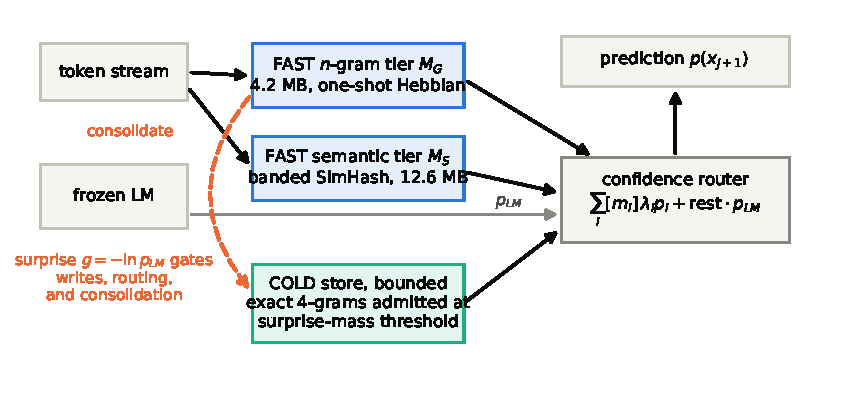
\includegraphics[width=0.9\linewidth]{figs/p3fig2_architecture.pdf}
\caption{The hierarchy. Fast Hebbian tiers absorb every token one-shot; high-surprise-mass $n$-grams distill into a bounded exact cold store; a per-position confidence router mixes the active tiers with the frozen LM. The surprise signal $g=-\ln p_{\mathrm{LM}}$ --- free at inference --- gates writes, routing and consolidation alike.}
\label{fig:arch}
\end{figure}

\paragraph{Contributions.}
\textbf{(C1)} The routed hierarchy improves on the two-tier router of \cite{router} with paired certainty on all three streams tested ($P = 1.000$ each), and on formulaic 500k-token text \emph{exceeds unbounded kNN-LM} while remaining fixed-plus-bounded in memory (\S\ref{sec:main}).
\textbf{(C2)} A consolidation Pareto: $\approx$10\% of the cold entries retain 92--94\% of the cold tier's value, and \emph{surprise-mass admission dominates count and random admission} wherever they differ --- the third measured role of the free surprise signal (\S\ref{sec:pareto}).
\textbf{(C3)} A demonstration that routing converts weak components into strong ones: the dictionary worth $+0.002$ alone contributes $+0.0195$ routed (\S\ref{sec:weak}).
\textbf{(C4)} Three documented methodological hazards of multi-tier evaluation, with verified remedies (\S\ref{sec:hazards}).

\section{Method}

\subsection{Tiers}

The fast tiers are exactly those of \cite{router}: $M_G \in \mathbb{R}^{4096\times256}$ addressed by sliding 4-gram bindings of token hypervectors; $M_S \in \mathbb{R}^{12288\times256}$ addressed by multi-resolution banded SimHash symbols over (whitened) hidden states; both written once per token with the amplitude rule of \cite{sillage} scaled by $g_j = \mathrm{clip}(-\ln p_{\mathrm{LM}}(x_{j+1}), 0, 5)$, both leaked with a 100k-token half-life.

The cold tier maintains, for each \emph{admitted} 4-gram, its successor counts; its prediction is the empirical successor distribution and its confidence is the gram's occurrence count. Admission policies compared, all capacity-matched to exactly $K$ grams (ties broken deterministically):
\emph{surprise-mass} (admit the top-$K$ grams by accumulated $\sum g$), \emph{count} (top-$K$ by occurrences), \emph{random} ($K$ grams at random). The unbounded store is the ceiling; removing the tier recovers the two-tier router as the control. Two stated idealizations, shared by all policies: an admitted gram answers with its full retrospective counts, and thresholds are calibrated to hit the target capacity (a deployed system would set them adaptively).

\subsection{Routing and tuning}

Per position, active tiers (those whose confidence clears a dev-quantile threshold) mix flatly:
$p = \sum_i \mathbf{1}[m_i]\, \lambda_i\, p_i + \max\!\big(0,\, 1 - \sum_i \mathbf{1}[m_i]\lambda_i\big)\, p_{\mathrm{LM}}$.
Tiers are tuned greedily --- each tier's (readout, $\lambda$, threshold) grid-searched with earlier tiers frozen --- and, because sequential tuning is order-sensitive (\S\ref{sec:hazards}), \emph{all tier orderings are tried and the best dev likelihood wins}. Every hyperparameter is selected on the first 20\% of the stream and frozen; results are reported on the remaining 80\% with 95\% block-bootstrap confidence intervals and paired tests on identical positions, following \cite{sillage}.

\section{Experiments}

Frozen GPT-2 124M; the three streams of \cite{sillage,router} where each tier has a known regime: \textsc{Bible} (KJV, 500k tokens, formulaic), \textsc{War and Peace} (500k, narrative), \textsc{Manuscripts} (36k, novel technical). The 500k protocol scores every 4th position; writes happen at every position; for coherence, \textsc{Manuscripts} uses the same stride here (its base and gains therefore differ numerically from the full-position numbers of \cite{sillage,router}; all comparisons within this paper share the protocol). Pipeline coherence is verified end-to-end: with the cold tier removed, the tuner reproduces the two-tier router's published numbers \emph{exactly} ($+0.0198$ on \textsc{Bible}, $+0.0191$ on \textsc{W\&P}).

\subsection{Main result: the hierarchy beats its parts --- and, on its home regime, kNN-LM}\label{sec:main}

\begin{table}[t]
\centering\small
\caption{Test $\dnll$ (nats) over frozen GPT-2. "Router" = two fast tiers \cite{router}; "+ cold" = full hierarchy with the unbounded cold tier; paired = block-bootstrap delta of the two on identical positions. Reference: unbounded kNN-LM under the same protocol.}
\label{tab:main}
\begin{tabular}{@{}lcccc@{}}
\toprule
stream & router (control) & + cold tier & paired $\Delta$ & kNN-LM (770\,MB)\\
\midrule
\textsc{Bible} (500k) & $+0.0198$ & $\mathbf{+0.0658}$ & $+0.0460$ \ci{0.0390}{0.0539} & $+0.0575$\\
\textsc{W\&P} (500k) & $+0.0191$ & $\mathbf{+0.0386}$ & $+0.0195$ \ci{0.0173}{0.0216} & $+0.0475$\\
\textsc{Manuscripts} & $+0.5269$ & $\mathbf{+0.6235}$ & $+0.0966$ \ci{0.0445}{0.1669} & ---\\
\bottomrule
\end{tabular}
\end{table}

Table~\ref{tab:main}: the cold tier adds a certain improvement on every stream ($P = 1.000$ in each paired test). On \textsc{Bible} the hierarchy reaches $+0.0658$ --- \textbf{above unbounded kNN-LM's $+0.0575$}, with two fixed matrices (16.8\,MB) plus a dictionary, against a 770\,MB store that scans itself at every query. On \textsc{W\&P} the hierarchy doubles the router and reaches 81\% of kNN-LM. The three mechanisms this line of work has benchmarked \emph{against} each other therefore compose: each tier dominates its regime, the router arbitrates, and no tier is dead weight anywhere.

\subsection{The consolidation Pareto: surprise selects what is worth keeping}\label{sec:pareto}

\begin{figure}[t]
\centering
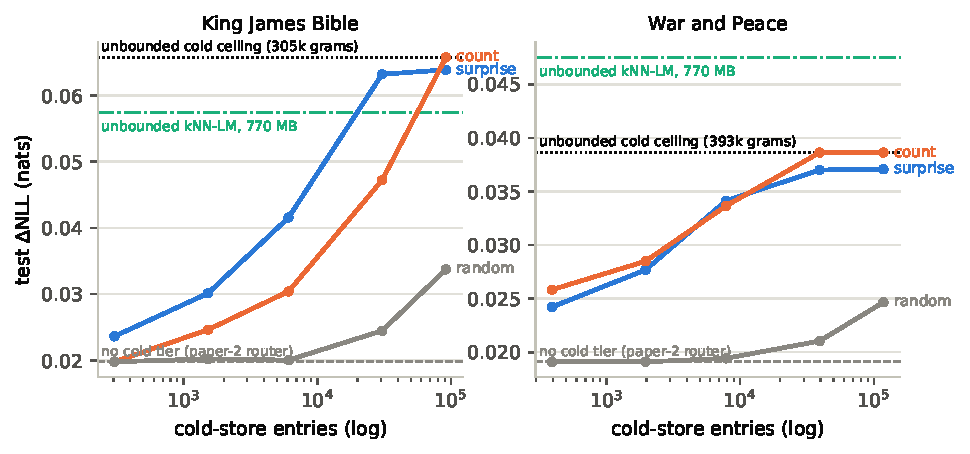
\includegraphics[width=\linewidth]{figs/p3fig1_pareto.pdf}
\caption{Consolidation Pareto: test $\dnll$ vs cold-store capacity (log scale) under three admission policies, with the no-cold control (dashed), the unbounded ceiling (dotted) and unbounded kNN-LM (dash-dotted). On formulaic text, surprise-mass admission crosses the kNN-LM line at $\approx$30k entries ($\approx$1\,MB of cold storage); count admission needs the near-full store; random admission fails.}
\label{fig:pareto}
\end{figure}

Figure~\ref{fig:pareto} is the paper's central measurement. Three findings.
\textbf{(i) A small consolidated store carries almost all the value.} At 10\% of the unbounded entries, surprise-mass admission retains 94\% of the cold tier's added gain on \textsc{Bible} ($+0.0632$ of $+0.0658$; 30.5k grams, $\approx$1\,MB) --- still above unbounded kNN-LM --- and 92\% on \textsc{W\&P}.
\textbf{(ii) Admission needs a signal, and surprise is the right one.} Random admission is flat at the control. Count admission fails exactly where selection matters most: at 0.1--2\% capacity on \textsc{Bible} it adds \emph{nothing} ($+0.0198 \to +0.0198/+0.0304$) while surprise admission already captures a third of the ceiling ($+0.0416$ at 2\%) --- the most frequent grams are function-word patterns the LM already predicts, whereas surprise mass $=$ frequency $\times$ difficulty selects grams that are \emph{recurrent and still surprising}, which is precisely what deserves consolidation. On \textsc{W\&P} the two informative policies are statistically equivalent (soft-repetition streams give counts and masses similar rankings); surprise admission is never worse.
\textbf{(iii) The same signal now does three jobs.} The gate $g$ that scales Hebbian writes \cite{sillage} and earns routing trust \cite{router} also ranks consolidation --- no new machinery, no learned parameters.

\subsection{Weak components become strong when routed}\label{sec:weak}

In \cite{sillage}, the standalone dictionary scored $+0.002$ on \textsc{W\&P} --- noise. Routed inside the hierarchy, gated by its own confidence (a minimum occurrence count) and mixed only where it knows something, the \emph{same} store contributes $+0.0195$ ($P = 1.000$), doubling the system. The converse of the paper-2 lesson completes the principle: key-level mixing lets a weak signal corrode a strong one, while score-level routing lets a weak component contribute exactly where it is strong. Arbitration, not raw component quality, is what compounds.

\subsection{Three hazards of multi-tier evaluation}\label{sec:hazards}

We document the pitfalls met while building this evaluation, each with its verified remedy.
\textbf{(a) Order sensitivity.} Sequential-residual tuning of the mixture underestimated the two-tier control by up to $4\times$ ($+0.0048$ vs $+0.0191$ on \textsc{W\&P}) until replaced by the flat mixture with dev-selected tier order; the fix was verified by \emph{exact} reproduction of the published router numbers from cached statistics.
\textbf{(b) Tie inflation.} Thresholding integer occurrence counts admits far more than the nominal capacity (massive ties), silently flattering the count policy; capacity-exact top-$K$ sets with deterministic tie-breaking restore a fair comparison --- and reversed an apparent policy ranking on one stream.
\textbf{(c) Non-stationary dev/test splits.} On \textsc{Manuscripts}, small-capacity cold tiers can improve dev while hurting test (dips of up to $-0.17$ nats below the control at 2\% capacity): the early stream under-represents the repetition structure of the rest. Acceptance margins or online validation are the remedies; we report the dips rather than hiding the configurations.

\section{Discussion}

\textbf{The complementary-systems reading.} The hierarchy operationalizes, in 30\,MB and with no gradients, the division of labor that complementary learning systems theory attributes to hippocampus and cortex \cite{mcclelland,kumaran}: fast, interference-limited, one-shot storage in front; slow, structured, capacity-managed storage behind; and a consolidation channel that transfers by \emph{value}, not recency. Our measured admission result sharpens the story: the value signal that works is not raw frequency but frequency weighted by prediction failure --- consolidate what keeps surprising you.

\textbf{Relation to learned test-time memories.} Titans and its relatives \cite{titans,ttr} learn surprise-gated writing and forgetting inside one neural memory; kNN-LM \cite{khandelwal2020} keeps everything and searches. The hierarchy occupies a third point: multiple fixed mechanisms, none learned, specialized by regime and arbitrated by confidence --- with the empirical bonus that on its home regime it outperforms the unbounded store outright.

\textbf{Limits.} One base model (GPT-2 124M) and three streams; the cold tier's two idealizations (retrospective serving, capacity-calibrated thresholds); no multi-seed replication of the hierarchy itself yet (its components are replicated in \cite{sillage,router}); and the \textsc{Manuscripts} dev/test dips show that consolidation thresholds inherit the non-stationarity problem documented in \cite{router}. The natural next steps are prospective consolidation with replay from the fast tier, adaptive thresholds, and the deployment setting the architecture obviously wants: a persistent assistant whose memory survives across sessions.

\section{Conclusion}

Three memory mechanisms that beat each other in different regimes become, once routed by confidence and consolidated by surprise, a single system that beats each of them everywhere tested --- including, on formulaic long streams, an unbounded kNN-LM store $25\times$ its size. The consolidation rule costs nothing: the model's own prediction loss, already gating every Hebbian write and every routing decision, also ranks what deserves permanence, and 10\% of the store chosen that way carries $\ge$92\% of its value. One signal, three tiers, no gradients.

\appendix

\section{Reproduction}

\texttt{hierarchy\_500k.py} runs one instrumented pass per stream (fast-tier statistics plus per-position gram count and surprise mass), caches it (\texttt{results/hier\_cache\_*.npz}), and evaluates every admission policy and capacity post hoc from the cache; \texttt{hier\_diag.py} is the coherence check against the published router numbers; \texttt{make\_figures\_p3.py} regenerates the figures. Grids, seeds, splits and statistics are identical to \cite{sillage,router}; hierarchy-specific settings: capacities $\{0.1, 0.5, 2, 10, 30\}\%$ of distinct grams, cold confidence gate $\in \{1,2,4\}$ occurrences, $\lambda_C \in \{0.05,\dots,0.85\}$.

\begin{thebibliography}{9}\small

\bibitem{sillage} A.~Sghairi. Sillage: Surprise-gated amplitude memory for frozen language models. Preprint, 2026.

\bibitem{router} A.~Sghairi. Route the scores, not the keys: Gradient-free semantic memory for frozen language models. Preprint, 2026.

\bibitem{khandelwal2020} U.~Khandelwal, O.~Levy, D.~Jurafsky, L.~Zettlemoyer, M.~Lewis. Generalization through memorization: Nearest neighbor language models. \emph{ICLR}, 2020.

\bibitem{titans} A.~Behrouz, P.~Zhong, V.~Mirrokni. Titans: Learning to memorize at test time. arXiv:2501.00663, 2025.

\bibitem{ttr} K.~A.~Wang, J.~Shi, E.~B.~Fox. Test-time regression: A unifying framework for designing sequence models with associative memory. arXiv:2501.12352, 2025.

\bibitem{mcclelland} J.~L.~McClelland, B.~L.~McNaughton, R.~C.~O'Reilly. Why there are complementary learning systems in the hippocampus and neocortex. \emph{Psychological Review}, 102(3):419--457, 1995.

\bibitem{kumaran} D.~Kumaran, D.~Hassabis, J.~L.~McClelland. What learning systems do intelligent agents need? \emph{Neuron}, 89(1):1134--1152, 2016.

\end{thebibliography}

\end{document}
